\documentclass{article}
\usepackage{amsmath}
\usepackage{graphicx}
\usepackage{booktabs}
\usepackage[colorlinks=true, allcolors=blue]{hyperref}
\usepackage[section]{placeins}


\title{Supplementary materials for: Pointing models for users operating under
different speed accuracy strategies  }
\author{Julien Gori}
\date{}
\begin{document}
\maketitle

\section{Pairplot for the EMG parameters of the JGP dataset (section 6.2)}

\begin{figure}[htbp]
    \centering
    \includegraphics[width=\textwidth]{img/pairplot_emg_jgp.pdf}
    \caption{Pairplot for the EMG parameters of the JGP dataset. Each panel shows the correlation between the two quantities. A panel between a quantity and itself represents that quantities' distribution.}
\end{figure}


% \section{Intraclass Correlation Coefficients (ICC) for the JGP dataset (Subsection 3.3)}
% \subsection{Pearson's $r$}
% \begin{center}
%     \begin{tabular}{lllrrrrrl}
%         \toprule
%           & Type  & Description             & ICC      & F        & df1 & df2 & pval     & CI95\%      \\
%         \midrule
%         0 & ICC1  & Single raters absolute  & 0.278121 & 2.541096 & 14  & 45  & 0.009083 & [0.04 0.59] \\
%         1 & ICC2  & Single random raters    & 0.284798 & 2.679707 & 14  & 42  & 0.006876 & [0.05 0.59] \\
%         2 & ICC3  & Single fixed raters     & 0.295738 & 2.679707 & 14  & 42  & 0.006876 & [0.05 0.61] \\
%         3 & ICC1k & Average raters absolute & 0.606469 & 2.541096 & 14  & 45  & 0.009083 & [0.15 0.85] \\
%         4 & ICC2k & Average random raters   & 0.614320 & 2.679707 & 14  & 42  & 0.006876 & [0.18 0.85] \\
%         5 & ICC3k & Average fixed raters    & 0.626825 & 2.679707 & 14  & 42  & 0.006876 & [0.18 0.86] \\
%         \bottomrule
%     \end{tabular}
% \end{center}

% \subsection{Spearman's $\rho$}
% \begin{center}
%     \begin{tabular}{lllrrrrrl}
%         \toprule
%           & Type  & Description             & ICC      & F        & df1 & df2 & pval     & CI95\%      \\
%         \midrule
%         0 & ICC1  & Single raters absolute  & 0.269582 & 2.476315 & 14  & 45  & 0.010850 & [0.03 0.58] \\
%         1 & ICC2  & Single random raters    & 0.272642 & 2.534710 & 14  & 42  & 0.010107 & [0.04 0.58] \\
%         2 & ICC3  & Single fixed raters     & 0.277288 & 2.534710 & 14  & 42  & 0.010107 & [0.04 0.59] \\
%         3 & ICC1k & Average raters absolute & 0.596174 & 2.476315 & 14  & 45  & 0.010850 & [0.12 0.85] \\
%         4 & ICC2k & Average random raters   & 0.599896 & 2.534710 & 14  & 42  & 0.010107 & [0.14 0.85] \\
%         5 & ICC3k & Average fixed raters    & 0.605478 & 2.534710 & 14  & 42  & 0.010107 & [0.13 0.85] \\
%         \bottomrule
%     \end{tabular}

% \end{center}


% \subsection{Kendall's $\tau$}
% \begin{center}
%     \begin{tabular}{lllrrrrrl}
%         \toprule
%           & Type  & Description             & ICC      & F        & df1 & df2 & pval     & CI95\%      \\
%         \midrule
%         0 & ICC1  & Single raters absolute  & 0.289989 & 2.633714 & 14  & 45  & 0.007048 & [0.05 0.6 ] \\
%         1 & ICC2  & Single random raters    & 0.291424 & 2.664110 & 14  & 42  & 0.007166 & [0.05 0.6 ] \\
%         2 & ICC3  & Single fixed raters     & 0.293799 & 2.664110 & 14  & 42  & 0.007166 & [0.05 0.6 ] \\
%         3 & ICC1k & Average raters absolute & 0.620308 & 2.633714 & 14  & 45  & 0.007048 & [0.18 0.86] \\
%         4 & ICC2k & Average random raters   & 0.621946 & 2.664110 & 14  & 42  & 0.007166 & [0.18 0.86] \\
%         5 & ICC3k & Average fixed raters    & 0.624640 & 2.664110 & 14  & 42  & 0.007166 & [0.18 0.86] \\
%         \bottomrule
%     \end{tabular}
% \end{center}


% \section{Effects of D and W on Pearson's $r$, Spearman's $\rho$ and Kendall's $\tau$}

% \subsection{Effect of D and W on Pearson's $r$}

% \begin{table}
%     \caption{Mixed Linear Model Regression Results}
%     \label{}
%     \begin{center}
%     \begin{tabular}{llll}
%     \hline
%     Model:            & MixedLM & Dependent Variable: & value     \\
%     No. Observations: & 180     & Method:             & REML      \\
%     No. Groups:       & 14      & Scale:              & 0.0096    \\
%     Min. group size:  & 12      & Log-Likelihood:     & 125.7111  \\
%     Max. group size:  & 24      & Converged:          & Yes       \\
%     Mean group size:  & 12.9    &                     &           \\
%     \hline
%     \end{tabular}
%     \end{center}
    
%     \begin{center}
%     \begin{tabular}{lrrrrrr}
%     \hline
%               &  Coef. & Std.Err. &      z & P$> |$z$|$ & [0.025 & 0.975]  \\
%     \hline
%     Intercept &  0.050 &    0.058 &  0.861 &       0.389 & -0.063 &  0.162  \\
%     D         &  0.000 &    0.000 &  1.065 &       0.287 & -0.000 &  0.000  \\
%     W         &  0.000 &    0.001 &  0.300 &       0.764 & -0.001 &  0.001  \\
%     D:W       & -0.000 &    0.000 & -1.707 &       0.088 & -0.000 &  0.000  \\
%     Group Var &  0.001 &    0.006 &        &             &        &         \\
%     \hline
%     \end{tabular}
%     \end{center}
%     \end{table}

% \subsection{Effect of D and W on Spearman's $\rho$}
% \begin{table}
%     \caption{Mixed Linear Model Regression Results}
%     \label{}
%     \begin{center}
%     \begin{tabular}{llll}
%     \hline
%     Model:            & MixedLM & Dependent Variable: & value    \\
%     No. Observations: & 180     & Method:             & REML     \\
%     No. Groups:       & 14      & Scale:              & 0.0156   \\
%     Min. group size:  & 12      & Log-Likelihood:     & 87.4109  \\
%     Max. group size:  & 24      & Converged:          & Yes      \\
%     Mean group size:  & 12.9    &                     &          \\
%     \hline
%     \end{tabular}
%     \end{center}
    
%     \begin{center}
%     \begin{tabular}{lrrrrrr}
%     \hline
%               &  Coef. & Std.Err. &      z & P$> |$z$|$ & [0.025 & 0.975]  \\
%     \hline
%     Intercept &  0.064 &    0.073 &  0.882 &       0.378 & -0.078 &  0.206  \\
%     D         &  0.000 &    0.000 &  0.420 &       0.675 & -0.000 &  0.000  \\
%     W         & -0.000 &    0.001 & -0.169 &       0.866 & -0.002 &  0.001  \\
%     D:W       & -0.000 &    0.000 & -0.647 &       0.517 & -0.000 &  0.000  \\
%     Group Var &  0.000 &    0.005 &        &             &        &         \\
%     \hline
%     \end{tabular}
%     \end{center}
%     \end{table}
    
% \subsection{Effect of D and W on Kendall's $\tau$}
% \begin{table}
%     \caption{Mixed Linear Model Regression Results}
%     \label{}
%     \begin{center}
%     \begin{tabular}{llll}
%     \hline
%     Model:            & MixedLM & Dependent Variable: & value     \\
%     No. Observations: & 180     & Method:             & REML      \\
%     No. Groups:       & 14      & Scale:              & 0.0107    \\
%     Min. group size:  & 12      & Log-Likelihood:     & 116.6185  \\
%     Max. group size:  & 24      & Converged:          & No        \\
%     Mean group size:  & 12.9    &                     &           \\
%     \hline
%     \end{tabular}
%     \end{center}
    
%     \begin{center}
%     \begin{tabular}{lrrrrrr}
%     \hline
%               &  Coef. & Std.Err. &      z & P$> |$z$|$ & [0.025 & 0.975]  \\
%     \hline
%     Intercept &  0.066 &    0.061 &  1.093 &       0.275 & -0.053 &  0.185  \\
%     D         &  0.000 &    0.000 &  0.820 &       0.412 & -0.000 &  0.000  \\
%     W         & -0.000 &    0.001 & -0.357 &       0.721 & -0.001 &  0.001  \\
%     D:W       & -0.000 &    0.000 & -0.926 &       0.354 & -0.000 &  0.000  \\
%     Group Var &  0.001 &    0.008 &        &             &        &         \\
%     \hline
%     \end{tabular}
%     \end{center}
%     \end{table}
    

% \section{Effects of D and W on the t-copulas parameters}

% \subsection{$\rho$}
% \subsubsection{Effect of W}
% \begin{table}
%     \caption{Mixed Linear Model Regression Results. Main effect W on $\rho$}
%     \label{}
%     \begin{center}
%     \begin{tabular}{llll}
%     \hline
%     Model:            & MixedLM & Dependent Variable: & $\rho$  \\
%     No. Observations: & 170     & Method:             & REML     \\
%     No. Groups:       & 15      & Scale:              & 0.0493   \\
%     Min. group size:  & 10      & Log-Likelihood:     & 4.9045   \\
%     Max. group size:  & 12      & Converged:          & No       \\
%     Mean group size:  & 11.3    &                     &          \\
%     \hline
%     \end{tabular}
%     \end{center}
    
%     \begin{center}
%     \begin{tabular}{lrrrrrr}
%     \hline
%               &  Coef. & Std.Err. &      z & P$> |$z$|$ & [0.025 & 0.975]  \\
%     \hline
%     Intercept & -0.115 &    0.066 & -1.745 &       0.081 & -0.245 &  0.014  \\
%     W         &  0.001 &    0.001 &  1.597 &       0.110 & -0.000 &  0.002  \\
%     Group Var &  0.001 &    0.013 &        &             &        &         \\
%     \hline
%     \end{tabular}
%     \end{center}
%     \end{table}

% \subsubsection{Effect of D}
% \begin{table}
%     \caption{Mixed Linear Model Regression Results. Main effect D on $\rho$}
%     \label{}
%     \begin{center}
%     \begin{tabular}{llll}
%     \hline
%     Model:            & MixedLM & Dependent Variable: & $\rho$  \\
%     No. Observations: & 170     & Method:             & REML     \\
%     No. Groups:       & 15      & Scale:              & 0.0501   \\
%     Min. group size:  & 10      & Log-Likelihood:     & 0.7523   \\
%     Max. group size:  & 12      & Converged:          & No       \\
%     Mean group size:  & 11.3    &                     &          \\
%     \hline
%     \end{tabular}
%     \end{center}
    
%     \begin{center}
%     \begin{tabular}{lrrrrrr}
%     \hline
%               &  Coef. & Std.Err. &      z & P$> |$z$|$ & [0.025 & 0.975]  \\
%     \hline
%     Intercept & -0.015 &    0.036 & -0.421 &       0.674 & -0.085 &  0.055  \\
%     D         &  0.000 &    0.000 &  0.035 &       0.972 & -0.000 &  0.000  \\
%     Group Var &  0.001 &    0.014 &        &             &        &         \\
%     \hline
%     \end{tabular}
%     \end{center}
%     \end{table}

% \subsubsection{Effect of ID}
% \begin{table}
%     \caption{Mixed Linear Model Regression Results. Main effect ID on $\rho$}
%     \label{}
%     \begin{center}
%     \begin{tabular}{llll}
%     \hline
%     Model:            & MixedLM & Dependent Variable: & $\rho$  \\
%     No. Observations: & 170     & Method:             & REML     \\
%     No. Groups:       & 15      & Scale:              & 0.0500   \\
%     Min. group size:  & 10      & Log-Likelihood:     & 7.1156   \\
%     Max. group size:  & 12      & Converged:          & No       \\
%     Mean group size:  & 11.3    &                     &          \\
%     \hline
%     \end{tabular}
%     \end{center}
    
%     \begin{center}
%     \begin{tabular}{lrrrrrr}
%     \hline
%               &  Coef. & Std.Err. &      z & P$> |$z$|$ & [0.025 & 0.975]  \\
%     \hline
%     Intercept &  0.017 &    0.062 &  0.267 &       0.790 & -0.106 &  0.139  \\
%     ID        & -0.010 &    0.019 & -0.514 &       0.607 & -0.048 &  0.028  \\
%     Group Var &  0.001 &    0.014 &        &             &        &         \\
%     \hline
%     \end{tabular}
%     \end{center}
%     \end{table}

% \subsection{$\nu$}
% \subsubsection{Effect of W}
% \begin{table}
%     \caption{Mixed Linear Model Regression Results. Main effect W on $\rho$}
%     \label{}
%     \begin{center}
%     \begin{tabular}{llll}
%     \hline
%     Model:            & MixedLM & Dependent Variable: & $\nu$         \\
%     No. Observations: & 170     & Method:             & REML            \\
%     No. Groups:       & 15      & Scale:              & 409148715.6844  \\
%     Min. group size:  & 10      & Log-Likelihood:     & -1917.0449      \\
%     Max. group size:  & 12      & Converged:          & No              \\
%     Mean group size:  & 11.3    &                     &                 \\
%     \hline
%     \end{tabular}
%     \end{center}
    
%     \begin{center}
%     \begin{tabular}{lrrrrrr}
%     \hline
%               &        Coef. & Std.Err. &      z & P$> |$z$|$ &   [0.025 &    0.975]  \\
%     \hline
%     Intercept &    13196.476 & 6151.321 &  2.145 &       0.032 & 1140.109 & 25252.842  \\
%     W         &      -56.842 &   60.155 & -0.945 &       0.345 & -174.744 &    61.060  \\
%     Group Var & 33506162.748 & 1171.304 &        &             &          &            \\
%     \hline
%     \end{tabular}
%     \end{center}
%     \end{table}
% \subsubsection{Effect of D}
% \begin{table}
%     \caption{Mixed Linear Model Regression Results. Main effect D on $\rho$}
%     \label{}
%     \begin{center}
%     \begin{tabular}{llll}
%     \hline
%     Model:            & MixedLM & Dependent Variable: & $\nu$         \\
%     No. Observations: & 170     & Method:             & REML            \\
%     No. Groups:       & 15      & Scale:              & 411033786.5680  \\
%     Min. group size:  & 10      & Log-Likelihood:     & -1920.3093      \\
%     Max. group size:  & 12      & Converged:          & No              \\
%     Mean group size:  & 11.3    &                     &                 \\
%     \hline
%     \end{tabular}
%     \end{center}
    
%     \begin{center}
%     \begin{tabular}{lrrrrrr}
%     \hline
%               &        Coef. & Std.Err. &      z & P$> |$z$|$ &   [0.025 &    0.975]  \\
%     \hline
%     Intercept &     8376.120 & 3510.011 &  2.386 &       0.017 & 1496.624 & 15255.616  \\
%     D         &       -0.788 &    3.491 & -0.226 &       0.821 &   -7.631 &     6.055  \\
%     Group Var & 33954748.337 & 1186.523 &        &             &          &            \\
%     \hline
%     \end{tabular}
%     \end{center}
%     \end{table}
% \subsubsection{Effect of ID}
% \begin{table}
%     \caption{Mixed Linear Model Regression Results. Main effect ID on $\rho$}
%     \label{}
%     \begin{center}
%     \begin{tabular}{llll}
%     \hline
%     Model:            & MixedLM & Dependent Variable: & $\nu$         \\
%     No. Observations: & 170     & Method:             & REML            \\
%     No. Groups:       & 15      & Scale:              & 411065779.3315  \\
%     Min. group size:  & 10      & Log-Likelihood:     & -1914.0843      \\
%     Max. group size:  & 12      & Converged:          & No              \\
%     Mean group size:  & 11.3    &                     &                 \\
%     \hline
%     \end{tabular}
%     \end{center}
    
%     \begin{center}
%     \begin{tabular}{lrrrrrr}
%     \hline
%               &        Coef. & Std.Err. &     z & P$> |$z$|$ &    [0.025 &    0.975]  \\
%     \hline
%     Intercept &     6579.024 & 5816.890 & 1.131 &       0.258 & -4821.870 & 17979.918  \\
%     ID        &      384.267 & 1768.291 & 0.217 &       0.828 & -3081.519 &  3850.053  \\
%     Group Var & 33916493.249 & 1184.884 &       &             &           &            \\
%     \hline
%     \end{tabular}
%     \end{center}
%     \end{table}

\section{Number of successful fits for the copula fits per (D,W) pair (Section 6.3)}

\begin{figure}[htbp]
    \centering
    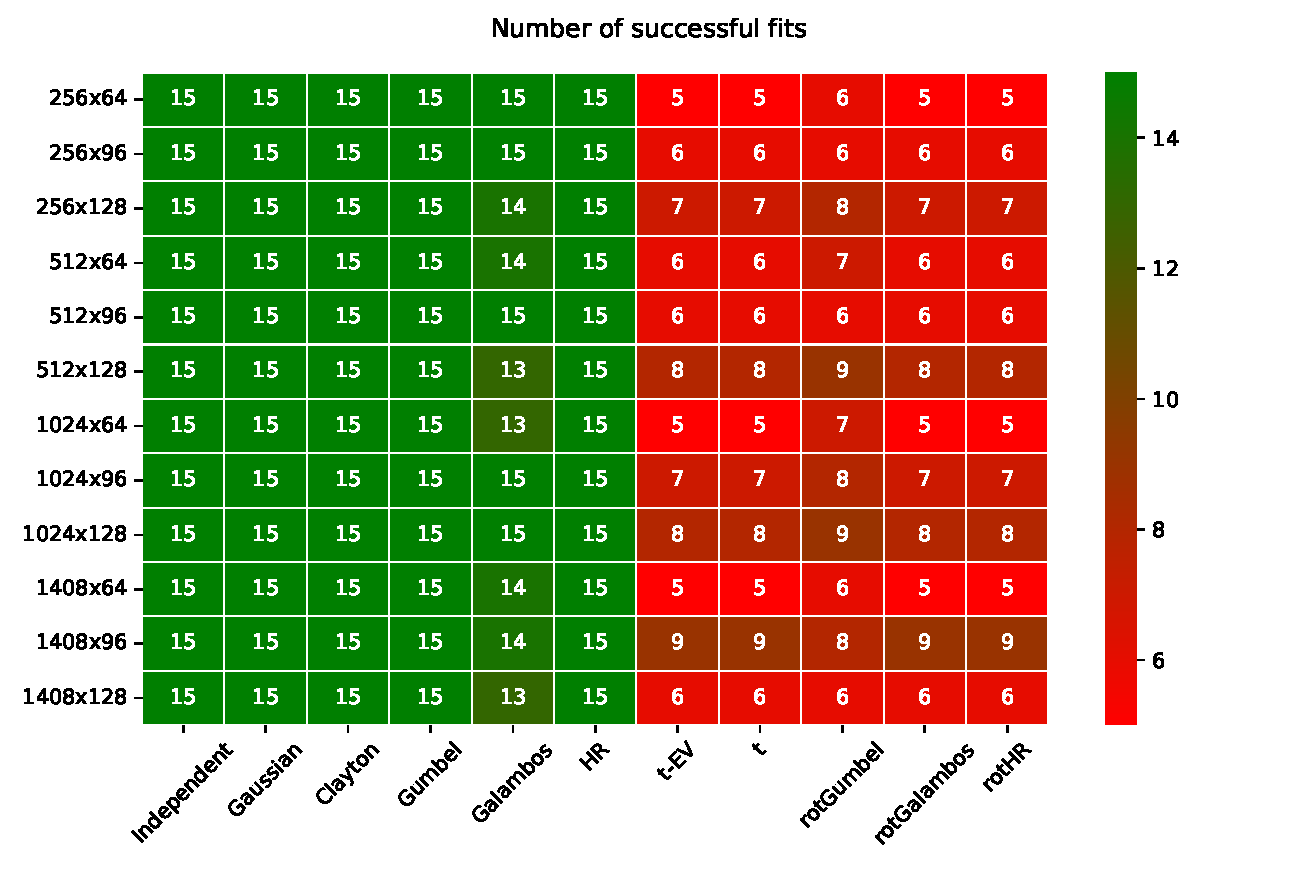
\includegraphics[width=.8\textwidth]{img/number_of_successful_copula_fits_jgp_dw.pdf}
    \caption{Number of successful fits for the copula fits per (D,W) pair. The number of unsuccessful fits is equally distributed over all conditions.}
\end{figure}


\section{Fits for ID$_e$ models as function of ID, W and D for the JGP dataset (section 6.4)}
\begin{table}
	\caption{Mixed Linear Model Regression Results for ID$_e$ on ID, W and D}
	\label{tab:fit_jgp_ide_id_full}
	\begin{center}
		\begin{tabular}{llll}
			\hline
			Model:            & MixedLM & Dependent Variable: & ide       \\
			No. Observations: & 714     & Method:             & REML      \\
			No. Groups:       & 15      & Scale:              & 0.0187    \\
			Min. group size:  & 46      & Log-Likelihood:     & 391.8485  \\
			Max. group size:  & 48      & Converged:          & Yes       \\
			Mean group size:  & 47.6    &                     &           \\
			\hline
			\end{tabular}
			\end{center}
			
			\begin{center}
			\begin{tabular}{lrrrrrr}
			\hline
					  &  Coef. & Std.Err. &      z & P$> |$z$|$ & [0.025 & 0.975]  \\
			\hline
			Intercept &  0.262 &    0.313 &  0.838 &       0.402 & -0.351 &  0.875  \\
			ID        &  0.846 &    0.115 &  7.331 &       0.000 &  0.620 &  1.072  \\
			w         & -0.992 &    1.835 & -0.541 &       0.589 & -4.588 &  2.604  \\
			ID:w      & -0.664 &    2.198 & -0.302 &       0.763 & -4.972 &  3.645  \\
			D         &  0.593 &    1.578 &  0.376 &       0.707 & -2.499 &  3.686  \\
			ID:D      & -0.042 &    0.202 & -0.206 &       0.837 & -0.438 &  0.355  \\
			w:D       &  5.022 &    5.825 &  0.862 &       0.389 & -6.395 & 16.440  \\
			ID:w:D    & -1.378 &    1.741 & -0.791 &       0.429 & -4.791 &  2.035  \\
			Group Var &  0.001 &    0.004 &        &             &        &         \\
			\hline
			\end{tabular}
			\end{center}
			\end{table}


\begin{table}
	\caption{Mixed Linear Model Regression Results for ID$_e$ on ID and W}
	\label{tab:fit_jgp_ide_id_w}
	\begin{center}
		\begin{tabular}{llll}
			\hline
			Model:            & MixedLM & Dependent Variable: & ide       \\
			No. Observations: & 714     & Method:             & REML      \\
			No. Groups:       & 15      & Scale:              & 0.0187    \\
			Min. group size:  & 46      & Log-Likelihood:     & 391.3947  \\
			Max. group size:  & 48      & Converged:          & Yes       \\
			Mean group size:  & 47.6    &                     &           \\
			\hline
			\end{tabular}
			\end{center}
			
			\begin{center}
			\begin{tabular}{lrrrrrr}
			\hline
					  & Coef. & Std.Err. &      z & P$> |$z$|$ & [0.025 & 0.975]  \\
			\hline
			Intercept & 0.016 &    0.077 &  0.211 &       0.833 & -0.134 &  0.167  \\
			ID        & 0.918 &    0.023 & 40.672 &       0.000 &  0.873 &  0.962  \\
			w         & 0.162 &    0.742 &  0.219 &       0.827 & -1.291 &  1.616  \\
			ID:w      & 0.379 &    0.232 &  1.637 &       0.102 & -0.075 &  0.833  \\
			Group Var & 0.001 &    0.004 &        &             &        &         \\
			\hline
			\end{tabular}
			\end{center}
			\end{table}
			
	
	\begin{table}
		\caption{Mixed Linear Model Regression Results for ID$_e$ on ID and D}
		\label{tab:fit_jgp_ide_id_D}
		\begin{center}
			\begin{tabular}{llll}
				\hline
				Model:            & MixedLM & Dependent Variable: & ide       \\
				No. Observations: & 714     & Method:             & REML      \\
				No. Groups:       & 15      & Scale:              & 0.0187    \\
				Min. group size:  & 46      & Log-Likelihood:     & 386.7450  \\
				Max. group size:  & 48      & Converged:          & Yes       \\
				Mean group size:  & 47.6    &                     &           \\
				\hline
				\end{tabular}
				\end{center}
				
				\begin{center}
				\begin{tabular}{lrrrrrr}
				\hline
						  &  Coef. & Std.Err. &      z & P$> |$z$|$ & [0.025 & 0.975]  \\
				\hline
				Intercept &  0.100 &    0.041 &  2.409 &       0.016 &  0.019 &  0.181  \\
				ID        &  0.890 &    0.017 & 51.507 &       0.000 &  0.856 &  0.924  \\
				D         &  0.296 &    0.067 &  4.423 &       0.000 &  0.165 &  0.427  \\
				ID:D      & -0.040 &    0.018 & -2.241 &       0.025 & -0.076 & -0.005  \\
				Group Var &  0.001 &    0.004 &        &             &        &         \\
				\hline
				\end{tabular}
				\end{center}
				\end{table}
				
			


% \section{Association measures for the GO dataset (Subsection 4.3)}

% \begin{figure}[htbp]
%     \centering
%     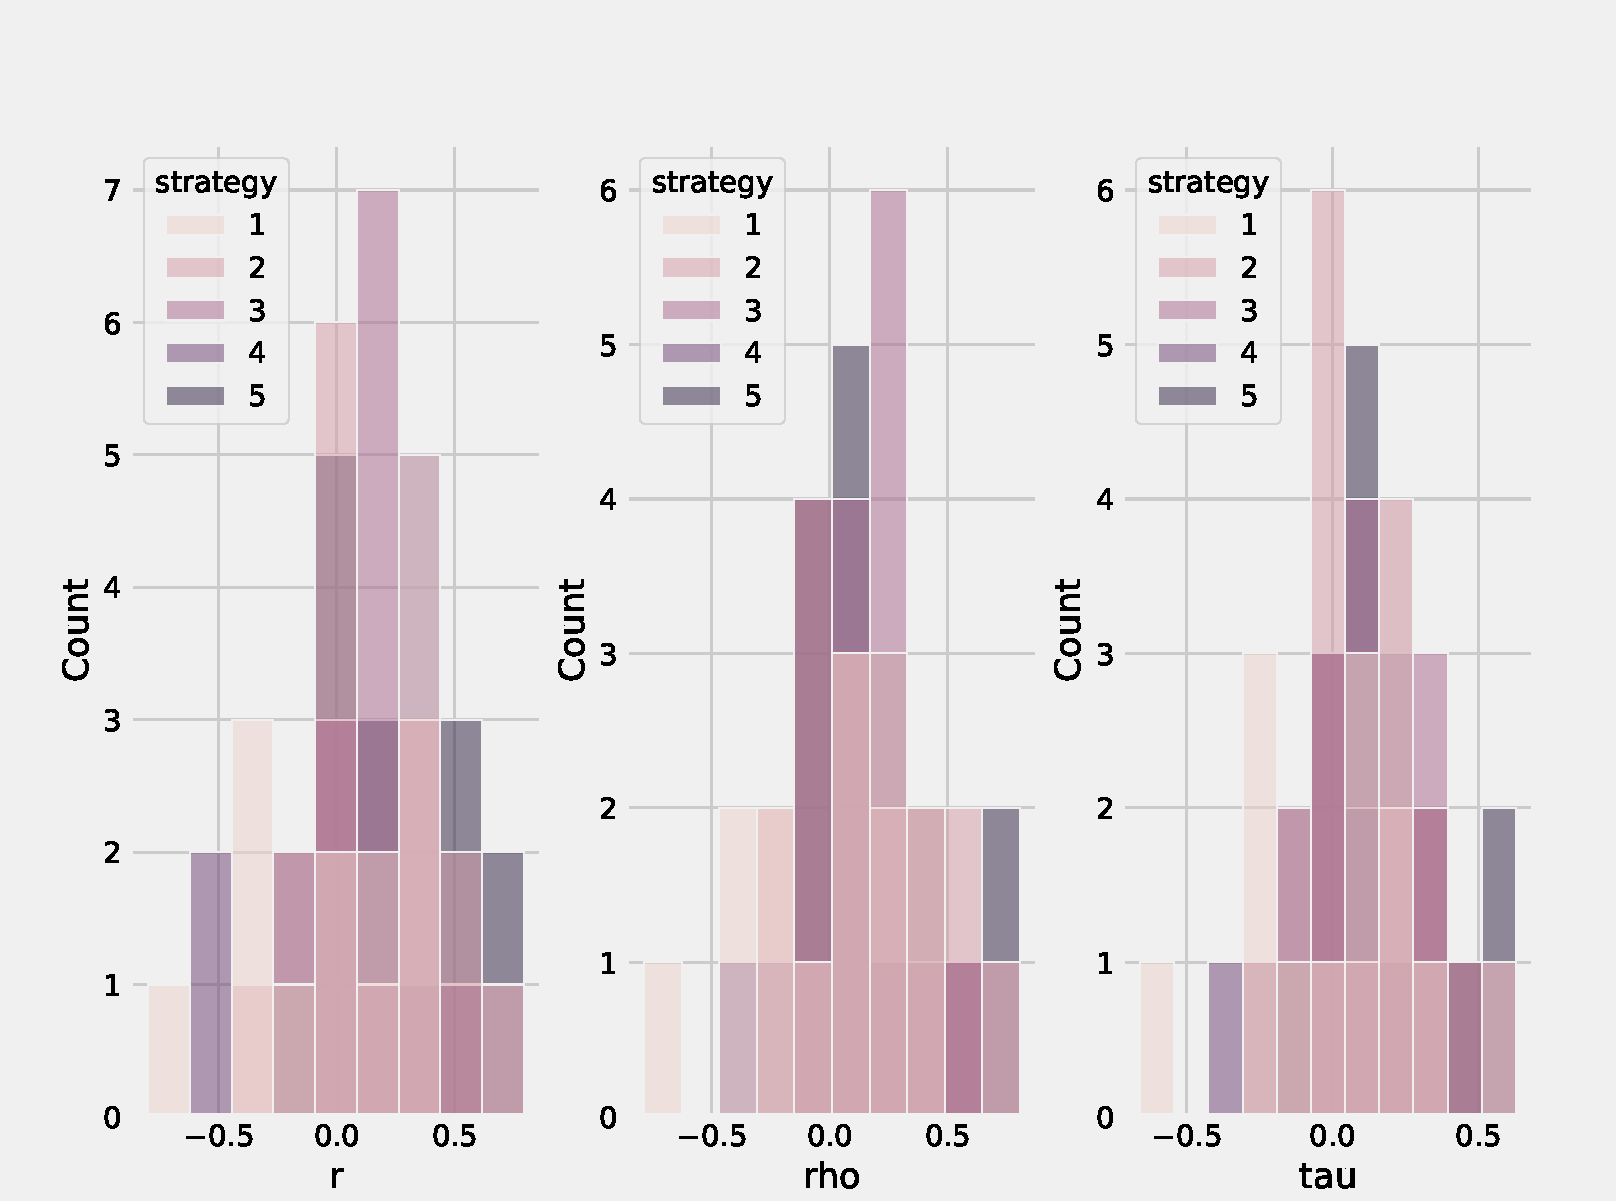
\includegraphics[width=.8\textwidth]{img/association_gop.pdf}
%     \caption{<caption>}
%     \label{<label>}
% \end{figure}
% \begin{table}
%     \centering
%     \caption{}
%     \begin{tabular}{lrrr}
%         \toprule
%                  & r        & rho      & tau      \\
%         strategy &          &          &          \\
%         \midrule
%         1        & 0.027881 & 0.034877 & 0.019789 \\
%         2        & 0.111236 & 0.116360 & 0.085362 \\
%         3        & 0.266716 & 0.262616 & 0.193317 \\
%         4        & 0.093823 & 0.107219 & 0.077531 \\
%         5        & 0.217365 & 0.226004 & 0.173897 \\
%         \bottomrule
%     \end{tabular}
% \end{table}

\section{$\rho$ values for the Gaussian copula (Section 6.5)}
\begin{table}[htbp]
	\centering
	\caption{Mean $\rho$ values of the Gaussian copula and associated t-statistics and p-values for the one way Student's t-test.}
	\begin{tabular}{lrrrrr}
		\toprule
		  Strategy & T-Statistic & P-Value & Mean & Count \\
		\midrule
		 1 (speed emph.) & 0.298 & 0.770 & 0.032 & 15 \\
		 2 (speed)& 1.67 & 0.118 & 0.134 & 15 \\
		 3 (balanced)& 6.91 & \textbf{\textless 0.001} & 0.321 & 15 \\
		 4 (accuracy) & 1.30 & 0.214 & 0.117 & 15 \\
		 5 (accuracy emph.)& 3.26 & \textbf{0.006} & 0.253 & 15 \\
		\bottomrule
		\end{tabular}
	\label{tab:gauss_corr}
\end{table}

\section{Pairplot for the EMG parameters for the GOP dataset (section 7.5)}

\begin{figure}[htbp]
    \centering
    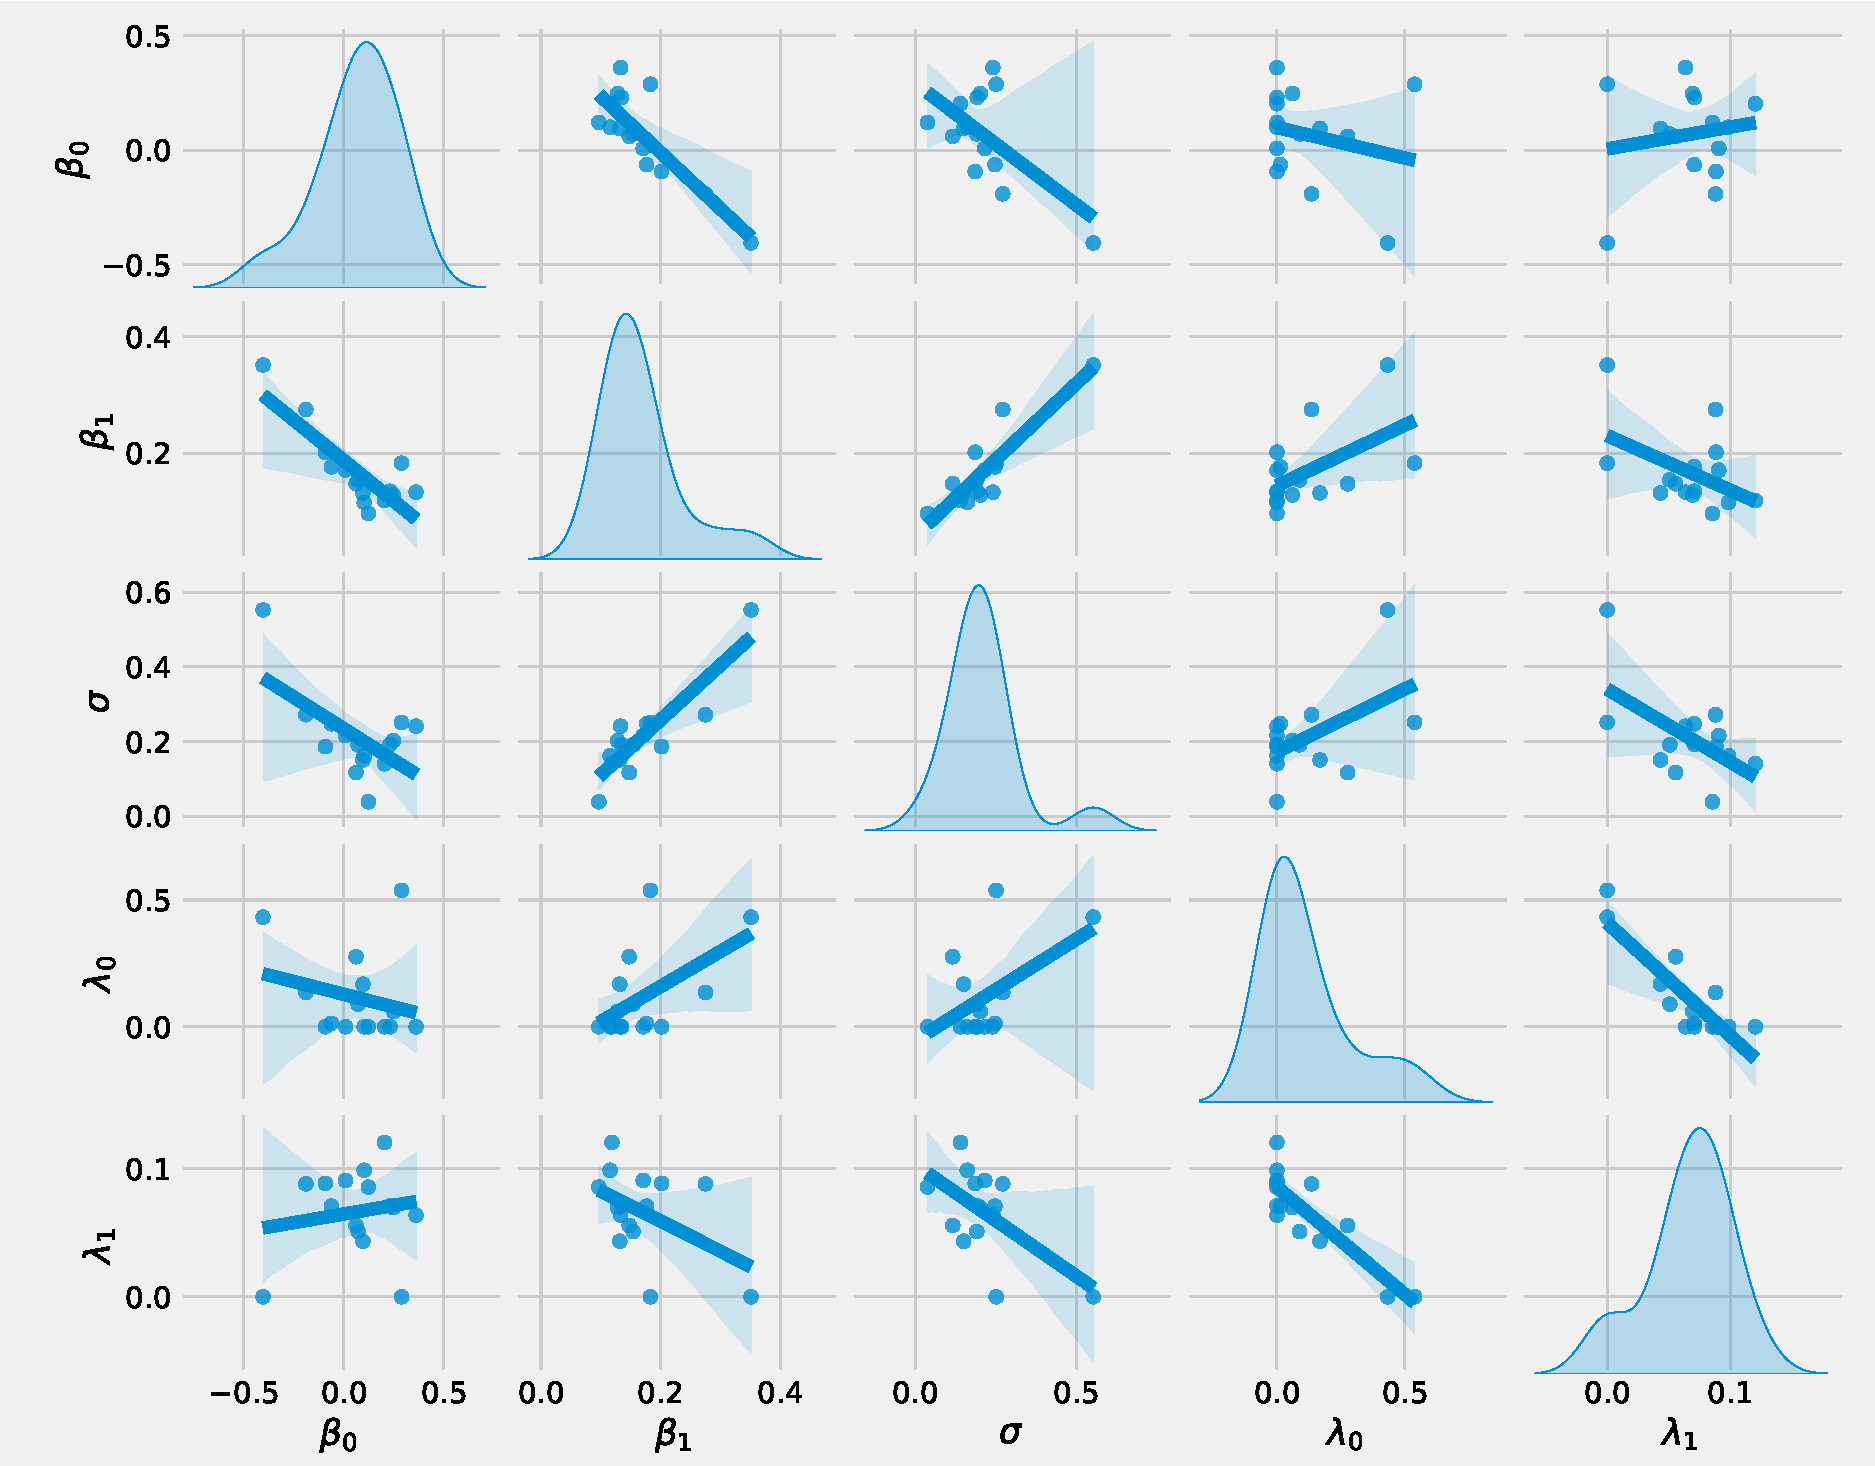
\includegraphics[width=\textwidth]{img/pairplot_gop.pdf}
    \caption{Pairplot for the EMG parameters for the GOP dataset. See the label of Figure 1.}
\end{figure}


\section{Violinplot for the Galambos Copula, GO dataset (section 7.6)}
\begin{figure}[htbp]
    \centering
    \includegraphics[width=.8\textwidth]{img/galambos_params.pdf}
    \caption{Parameter of the Galambos copula in the balanced condition in the GO dataset.}
    \label{<label>}
\end{figure}


\section{Parameters of the t-copula, GO dataset (section 7.6)}
\begin{figure}[htbp]
    \centering
    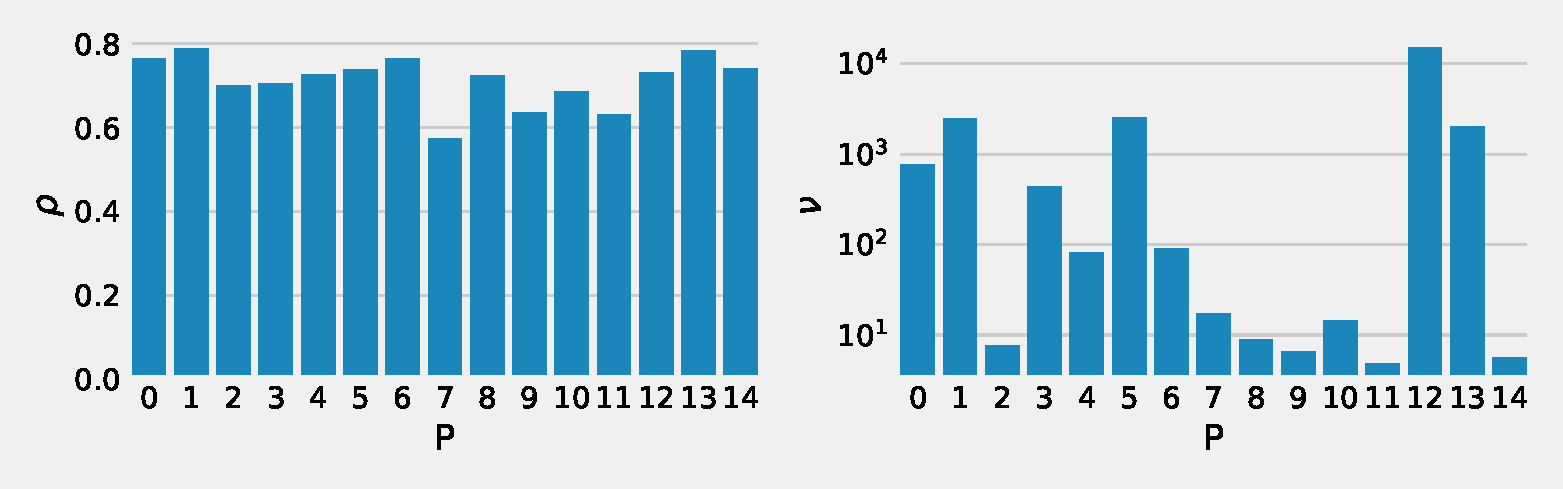
\includegraphics[width=\textwidth]{img/t_cop_parameters.pdf}
    \caption{Parameters of the t-copula (GO dataset). Left: $\rho$, right: $\nu$.}
\end{figure}


% \section{Linear fits for the Gaussian bivariate fit per strategy for the GO dataset (Subsection 4.5)}
% \subsection{$\mu_i = \text{const} + x_1\,\text{strategy}$}
% \begin{center}
%     \begin{tabular}{lclc}
%         \toprule
%         \textbf{Dep. Variable:}    & y                & \textbf{  R-squared:         } & 0.934   \\
%         \textbf{Model:}            & OLS              & \textbf{  Adj. R-squared:    } & 0.912   \\
%         \textbf{Method:}           & Least Squares    & \textbf{  F-statistic:       } & 42.58   \\
%         \textbf{Date:}             & Tue, 10 Sep 2024 & \textbf{  Prob (F-statistic):} & 0.00731 \\
%         \textbf{Time:}             & 16:31:51         & \textbf{  Log-Likelihood:    } & 3.4797  \\
%         \textbf{No. Observations:} & 5                & \textbf{  AIC:               } & -2.959  \\
%         \textbf{Df Residuals:}     & 3                & \textbf{  BIC:               } & -3.741  \\
%         \textbf{Df Model:}         & 1                & \textbf{                     } &         \\
%         \textbf{Covariance Type:}  & nonrobust        & \textbf{                     } &         \\
%         \bottomrule
%     \end{tabular}
%     \begin{tabular}{lcccccc}
%                        & \textbf{coef} & \textbf{std err} & \textbf{t} & \textbf{P$> |$t$|$} & \textbf{[0.025} & \textbf{0.975]} \\
%         \midrule
%         \textbf{const} & 1.2957        & 0.070            & 18.602     & 0.000               & 1.074           & 1.517           \\
%         \textbf{x1}    & 0.6428        & 0.099            & 6.525      & 0.007               & 0.329           & 0.956           \\
%         \bottomrule
%     \end{tabular}
%     \begin{tabular}{lclc}
%         \textbf{Omnibus:}       & nan   & \textbf{  Durbin-Watson:     } & 1.778 \\
%         \textbf{Prob(Omnibus):} & nan   & \textbf{  Jarque-Bera (JB):  } & 0.441 \\
%         \textbf{Skew:}          & 0.048 & \textbf{  Prob(JB):          } & 0.802 \\
%         \textbf{Kurtosis:}      & 1.548 & \textbf{  Cond. No.          } & 1.41  \\
%         \bottomrule
%     \end{tabular}
%     %\caption{OLS Regression Results}
% \end{center}

% Notes: \newline
% [1] Standard Errors assume that the covariance matrix of the errors is correctly specified.



% \subsection{$\mu_t = \text{const} + x_1\,\text{strategy}$}
% \begin{center}
%     \begin{tabular}{lclc}
%         \toprule
%         \textbf{Dep. Variable:}    & y                & \textbf{  R-squared:         } & 0.934   \\
%         \textbf{Model:}            & OLS              & \textbf{  Adj. R-squared:    } & 0.912   \\
%         \textbf{Method:}           & Least Squares    & \textbf{  F-statistic:       } & 42.58   \\
%         \textbf{Date:}             & Tue, 10 Sep 2024 & \textbf{  Prob (F-statistic):} & 0.00731 \\
%         \textbf{Time:}             & 16:31:51         & \textbf{  Log-Likelihood:    } & 3.4797  \\
%         \textbf{No. Observations:} & 5                & \textbf{  AIC:               } & -2.959  \\
%         \textbf{Df Residuals:}     & 3                & \textbf{  BIC:               } & -3.741  \\
%         \textbf{Df Model:}         & 1                & \textbf{                     } &         \\
%         \textbf{Covariance Type:}  & nonrobust        & \textbf{                     } &         \\
%         \bottomrule
%     \end{tabular}
%     \begin{tabular}{lcccccc}
%                        & \textbf{coef} & \textbf{std err} & \textbf{t} & \textbf{P$> |$t$|$} & \textbf{[0.025} & \textbf{0.975]} \\
%         \midrule
%         \textbf{const} & 1.2957        & 0.070            & 18.602     & 0.000               & 1.074           & 1.517           \\
%         \textbf{x1}    & 0.6428        & 0.099            & 6.525      & 0.007               & 0.329           & 0.956           \\
%         \bottomrule
%     \end{tabular}
%     \begin{tabular}{lclc}
%         \textbf{Omnibus:}       & nan   & \textbf{  Durbin-Watson:     } & 1.778 \\
%         \textbf{Prob(Omnibus):} & nan   & \textbf{  Jarque-Bera (JB):  } & 0.441 \\
%         \textbf{Skew:}          & 0.048 & \textbf{  Prob(JB):          } & 0.802 \\
%         \textbf{Kurtosis:}      & 1.548 & \textbf{  Cond. No.          } & 1.41  \\
%         \bottomrule
%     \end{tabular}
%     %\caption{OLS Regression Results}
% \end{center}

% Notes: \newline
% [1] Standard Errors assume that the covariance matrix of the errors is correctly specified.


% \subsection{$\sigma_i = \text{const} + x_1\,\text{strategy}$}

% \begin{center}
%     \begin{tabular}{lclc}
%         \toprule
%         \textbf{Dep. Variable:}    & y                & \textbf{  R-squared:         } & 0.590   \\
%         \textbf{Model:}            & OLS              & \textbf{  Adj. R-squared:    } & 0.453   \\
%         \textbf{Method:}           & Least Squares    & \textbf{  F-statistic:       } & 4.317   \\
%         \textbf{Date:}             & Tue, 10 Sep 2024 & \textbf{  Prob (F-statistic):} & 0.129   \\
%         \textbf{Time:}             & 16:31:51         & \textbf{  Log-Likelihood:    } & 1.6774  \\
%         \textbf{No. Observations:} & 5                & \textbf{  AIC:               } & 0.6452  \\
%         \textbf{Df Residuals:}     & 3                & \textbf{  BIC:               } & -0.1360 \\
%         \textbf{Df Model:}         & 1                & \textbf{                     } &         \\
%         \textbf{Covariance Type:}  & nonrobust        & \textbf{                     } &         \\
%         \bottomrule
%     \end{tabular}
%     \begin{tabular}{lcccccc}
%                        & \textbf{coef} & \textbf{std err} & \textbf{t} & \textbf{P$> |$t$|$} & \textbf{[0.025} & \textbf{0.975]} \\
%         \midrule
%         \textbf{const} & 1.0564        & 0.100            & 10.576     & 0.002               & 0.739           & 1.374           \\
%         \textbf{x1}    & 0.2935        & 0.141            & 2.078      & 0.129               & -0.156          & 0.743           \\
%         \bottomrule
%     \end{tabular}
%     \begin{tabular}{lclc}
%         \textbf{Omnibus:}       & nan    & \textbf{  Durbin-Watson:     } & 1.799 \\
%         \textbf{Prob(Omnibus):} & nan    & \textbf{  Jarque-Bera (JB):  } & 0.816 \\
%         \textbf{Skew:}          & -0.387 & \textbf{  Prob(JB):          } & 0.665 \\
%         \textbf{Kurtosis:}      & 1.178  & \textbf{  Cond. No.          } & 1.41  \\
%         \bottomrule
%     \end{tabular}
%     %\caption{OLS Regression Results}
% \end{center}

% Notes: \newline
% [1] Standard Errors assume that the covariance matrix of the errors is correctly specified.

% \subsection{$\sigma_t = \text{const} + x_1\,\text{strategy}$}

% \begin{center}
%     \begin{tabular}{lclc}
%         \toprule
%         \textbf{Dep. Variable:}    & y                & \textbf{  R-squared:         } & 0.681  \\
%         \textbf{Model:}            & OLS              & \textbf{  Adj. R-squared:    } & 0.574  \\
%         \textbf{Method:}           & Least Squares    & \textbf{  F-statistic:       } & 6.396  \\
%         \textbf{Date:}             & Tue, 10 Sep 2024 & \textbf{  Prob (F-statistic):} & 0.0855 \\
%         \textbf{Time:}             & 16:31:52         & \textbf{  Log-Likelihood:    } & 9.2180 \\
%         \textbf{No. Observations:} & 5                & \textbf{  AIC:               } & -14.44 \\
%         \textbf{Df Residuals:}     & 3                & \textbf{  BIC:               } & -15.22 \\
%         \textbf{Df Model:}         & 1                & \textbf{                     } &        \\
%         \textbf{Covariance Type:}  & nonrobust        & \textbf{                     } &        \\
%         \bottomrule
%     \end{tabular}
%     \begin{tabular}{lcccccc}
%                        & \textbf{coef} & \textbf{std err} & \textbf{t} & \textbf{P$> |$t$|$} & \textbf{[0.025} & \textbf{0.975]} \\
%         \midrule
%         \textbf{const} & 0.3852        & 0.022            & 17.424     & 0.000               & 0.315           & 0.456           \\
%         \textbf{x1}    & 0.0791        & 0.031            & 2.529      & 0.085               & -0.020          & 0.179           \\
%         \bottomrule
%     \end{tabular}
%     \begin{tabular}{lclc}
%         \textbf{Omnibus:}       & nan   & \textbf{  Durbin-Watson:     } & 1.787 \\
%         \textbf{Prob(Omnibus):} & nan   & \textbf{  Jarque-Bera (JB):  } & 0.759 \\
%         \textbf{Skew:}          & 0.358 & \textbf{  Prob(JB):          } & 0.684 \\
%         \textbf{Kurtosis:}      & 1.231 & \textbf{  Cond. No.          } & 1.41  \\
%         \bottomrule
%     \end{tabular}
%     %\caption{OLS Regression Results}
% \end{center}

% Notes: \newline
% [1] Standard Errors assume that the covariance matrix of the errors is correctly specified.

% \subsection{$\rho = \text{const} + x_1\,\text{strategy}$}

% \begin{center}
%     \begin{tabular}{lclc}
%         \toprule
%         \textbf{Dep. Variable:}    & y                & \textbf{  R-squared:         } & 0.565  \\
%         \textbf{Model:}            & OLS              & \textbf{  Adj. R-squared:    } & 0.420  \\
%         \textbf{Method:}           & Least Squares    & \textbf{  F-statistic:       } & 3.896  \\
%         \textbf{Date:}             & Tue, 10 Sep 2024 & \textbf{  Prob (F-statistic):} & 0.143  \\
%         \textbf{Time:}             & 16:31:52         & \textbf{  Log-Likelihood:    } & 3.0488 \\
%         \textbf{No. Observations:} & 5                & \textbf{  AIC:               } & -2.098 \\
%         \textbf{Df Residuals:}     & 3                & \textbf{  BIC:               } & -2.879 \\
%         \textbf{Df Model:}         & 1                & \textbf{                     } &        \\
%         \textbf{Covariance Type:}  & nonrobust        & \textbf{                     } &        \\
%         \bottomrule
%     \end{tabular}
%     \begin{tabular}{lcccccc}
%                        & \textbf{coef} & \textbf{std err} & \textbf{t} & \textbf{P$> |$t$|$} & \textbf{[0.025} & \textbf{0.975]} \\
%         \midrule
%         \textbf{const} & 0.3447        & 0.076            & 4.539      & 0.020               & 0.103           & 0.586           \\
%         \textbf{x1}    & 0.2119        & 0.107            & 1.974      & 0.143               & -0.130          & 0.554           \\
%         \bottomrule
%     \end{tabular}
%     \begin{tabular}{lclc}
%         \textbf{Omnibus:}       & nan   & \textbf{  Durbin-Watson:     } & 1.648 \\
%         \textbf{Prob(Omnibus):} & nan   & \textbf{  Jarque-Bera (JB):  } & 0.479 \\
%         \textbf{Skew:}          & 0.485 & \textbf{  Prob(JB):          } & 0.787 \\
%         \textbf{Kurtosis:}      & 1.833 & \textbf{  Cond. No.          } & 1.41  \\
%         \bottomrule
%     \end{tabular}
%     %\caption{OLS Regression Results}
% \end{center}

% Notes: \newline
% [1] Standard Errors assume that the covariance matrix of the errors is correctly specified.

\section{Parameter values for the t-copula for the YKORM dataset (section 7.6)}
\begin{figure}[htbp]
	\centering
	\includegraphics[width=.8\textwidth]{../img/rho_nu_SP_yamanaka.pdf}
	\caption{Parameters of the t-copula for different strategies.}
	\label{fig:rho_nu}
\end{figure}


\section{Parameter values for the Gaussian copula for the YORMK dataset (section 8.6)}

\begin{figure}[htbp]
    \centering
    \includegraphics[width=.8\textwidth]{img/rho_DW_yamanaka}
    \caption{Gaussian copula parameters for different D and W conditions}
    \label{fig:rho_DW}
\end{figure}

\begin{table}[htbp]
    \begin{center}
        \caption{Effect of D and W on $\rho$. The statistical model evaluated is $\rho \sim$  W*D + (1$|$participants).}
        \begin{tabular}{lrrrrrr}
        \hline
                  &  Coef. & Std.Err. &      z & P$> |$z$|$ & [0.025 & 0.975]  \\
        \hline
        Intercept &  0.413 &    0.123 &  3.372 &       0.001 &  0.173 &  0.653  \\
        W         &  0.002 &    0.003 &  0.756 &       0.449 & -0.003 &  0.007  \\
        D         & -0.000 &    0.000 & -0.033 &       0.974 & -0.000 &  0.000  \\
        W:D       & -0.000 &    0.000 & -0.790 &       0.430 & -0.000 &  0.000  \\
        Group Var &  0.040 &    0.125 &        &             &        &         \\
        \hline
        \end{tabular}
        \end{center}
        
    \caption{<caption>}
    \label{<label>}
\end{table}

\section{Parameter values for the Galambos copula (Section 8.4.2)}
\begin{figure}[htbp]
	\centering
	\includegraphics[width=.5\textwidth]{../img/theta_w_pdd.pdf}
	\caption{The Galambos copula's parameter $\theta$ plotted against $W$.}
	\label{}
\end{figure}

\section{Replications of Figure 7 with different seeds (Subsection 11.1)}

\begin{figure}[htbp]
    \centering
    \makebox[\textwidth]{
        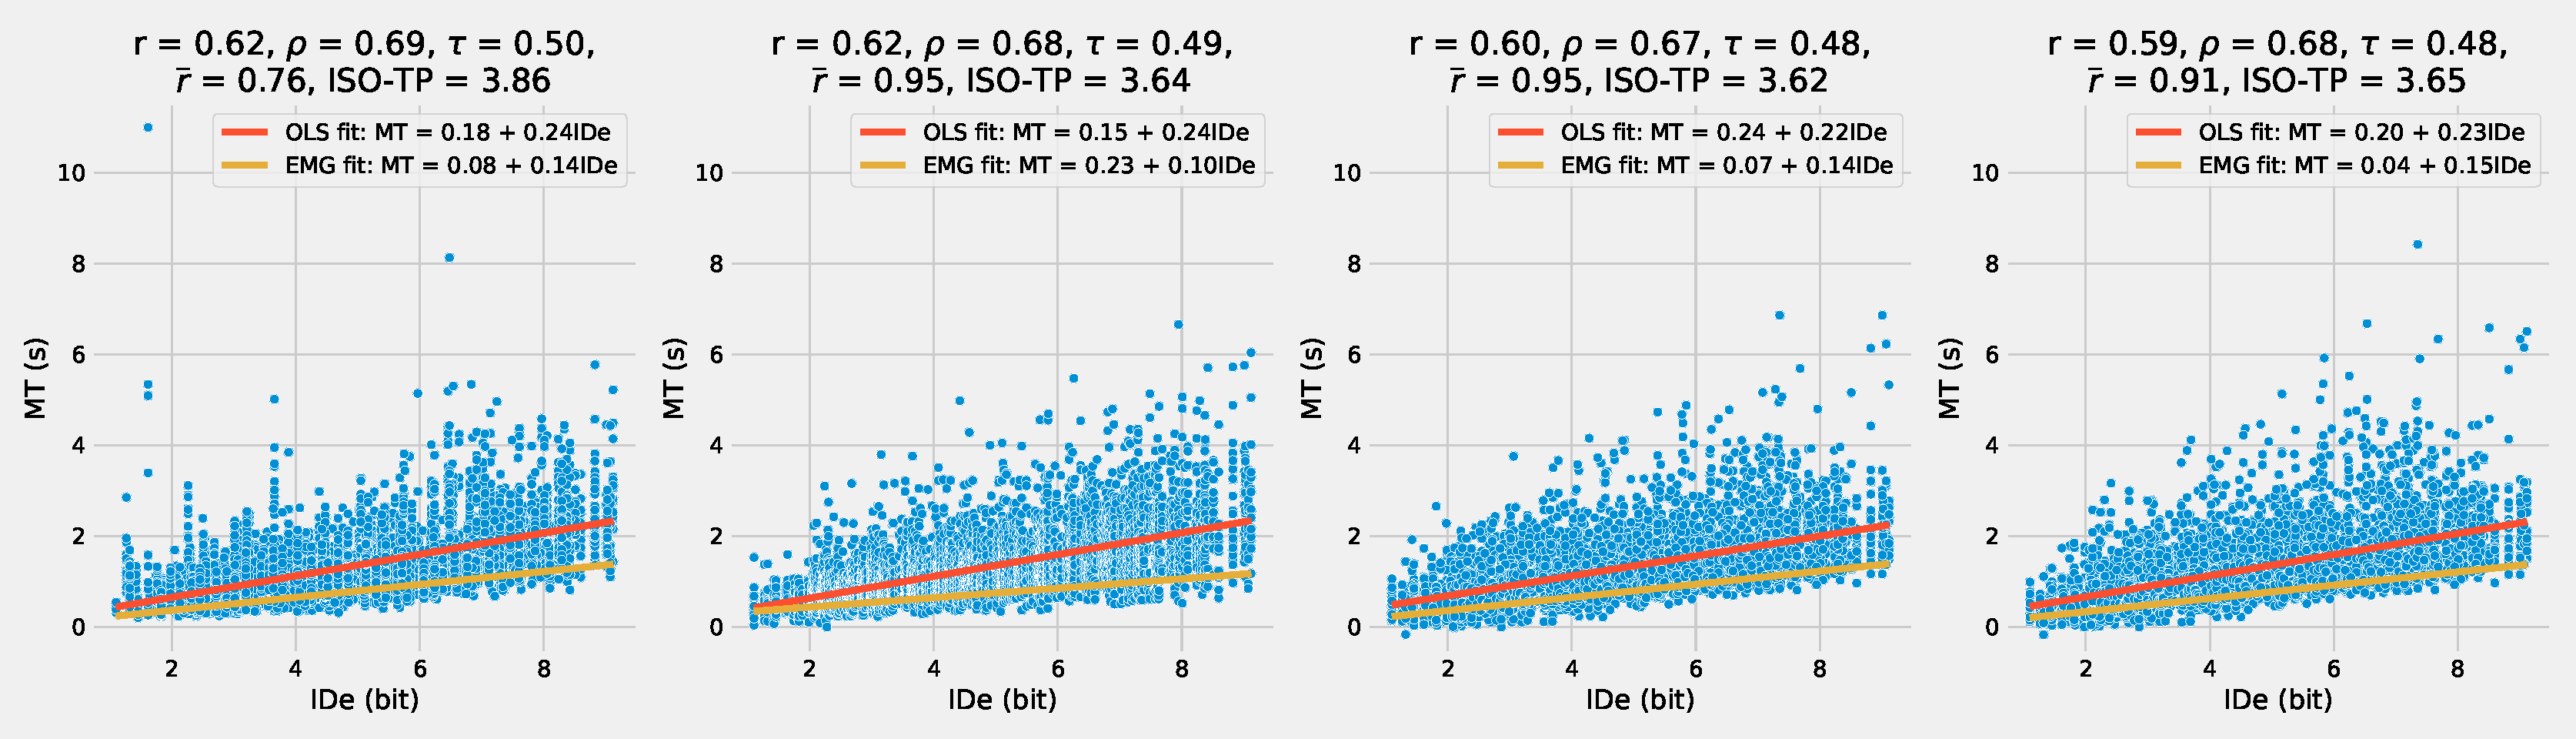
\includegraphics[width=1.3\textwidth]{img/method_consistency_seed777.pdf}
    }
    \caption{Seed = 777}
\end{figure}
\begin{figure}[htbp]
    \centering
    \makebox[\textwidth]{
        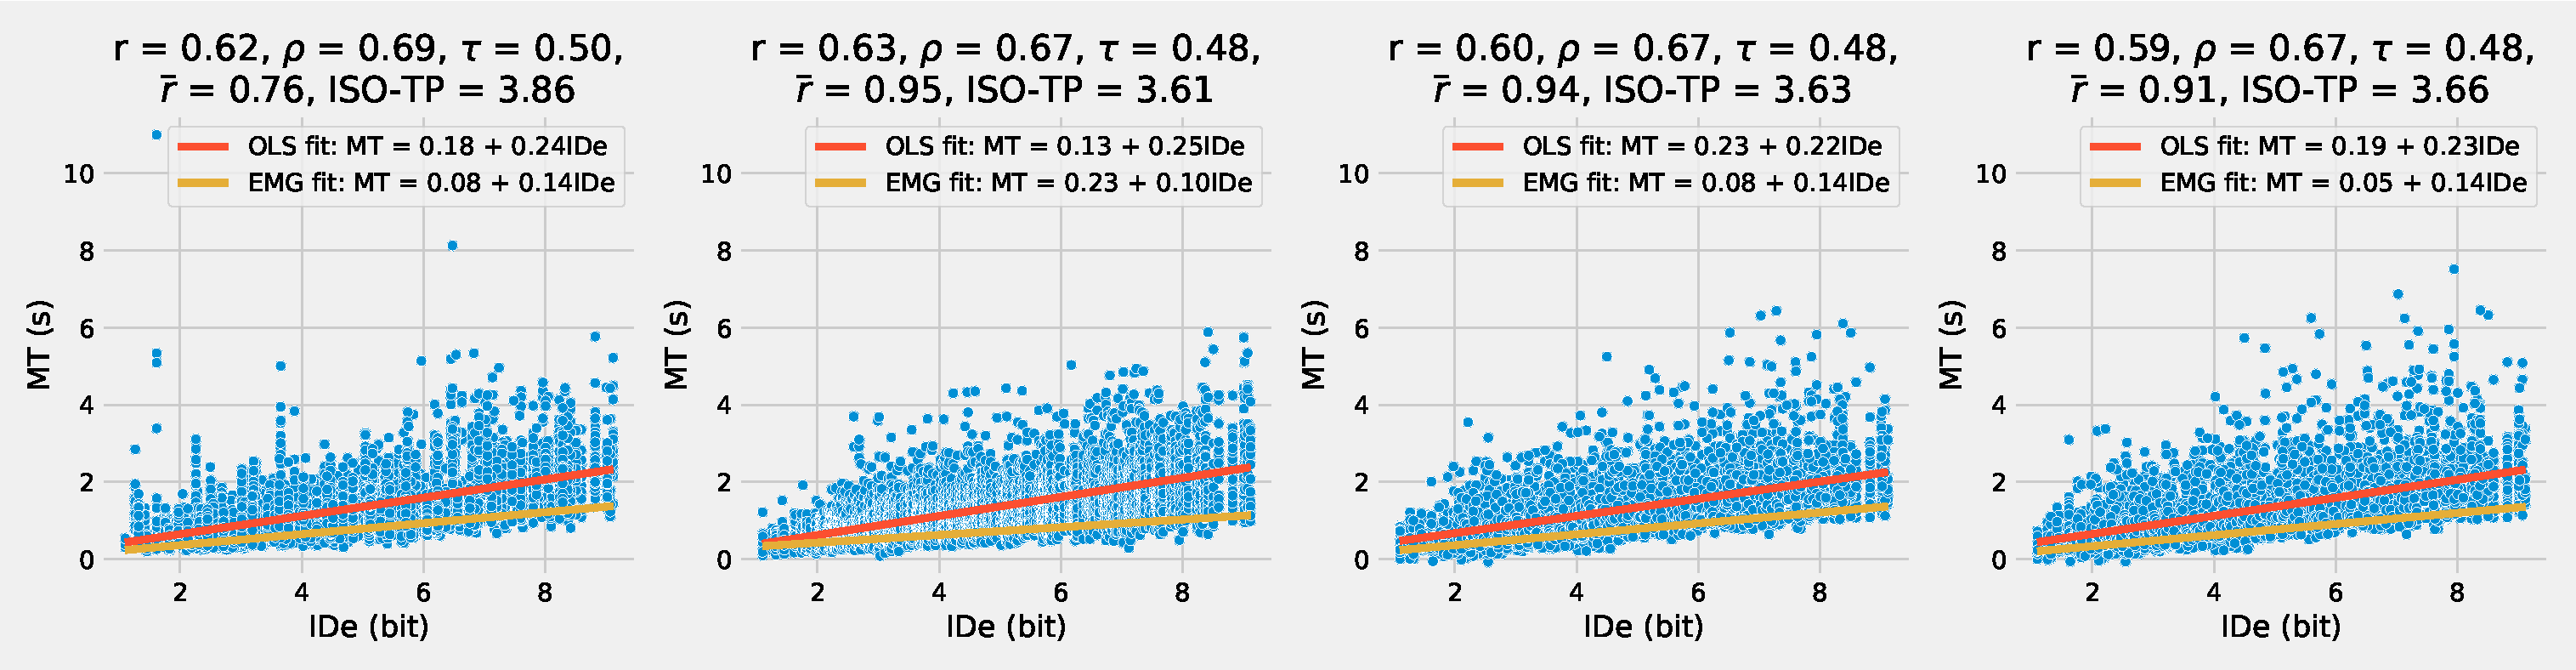
\includegraphics[width=1.3\textwidth]{img/method_consistency_seed999.pdf}
    }
    \caption{Seed = 999}
\end{figure}
\begin{figure}[htbp]
    \centering
    \makebox[\textwidth]{
        \includegraphics[width=1.3\textwidth]{img/method_consistency_seedNone.pdf}
    }
    \caption{Seed = None}
\end{figure}

\section{Correction on $\beta_0$ instead of $\lambda_1$ for Model 3 (Subsection 11.1)}

\begin{figure}[htbp]
    \centering
    \makebox[\textwidth]{
        \includegraphics[width=1.3\textwidth]{img/method_consistency_correct_beta.pdf}
    }
    \caption{Effect of correction $beta_0$ instead of $\lambda_1$ for model 3.}
\end{figure}


\section{Participant internal consistency concerning strategies (section 13.3)}

\begin{figure}[htbp]
    \centering
    \includegraphics[width=.48\textwidth]{img/fitts_gop_1.pdf}
    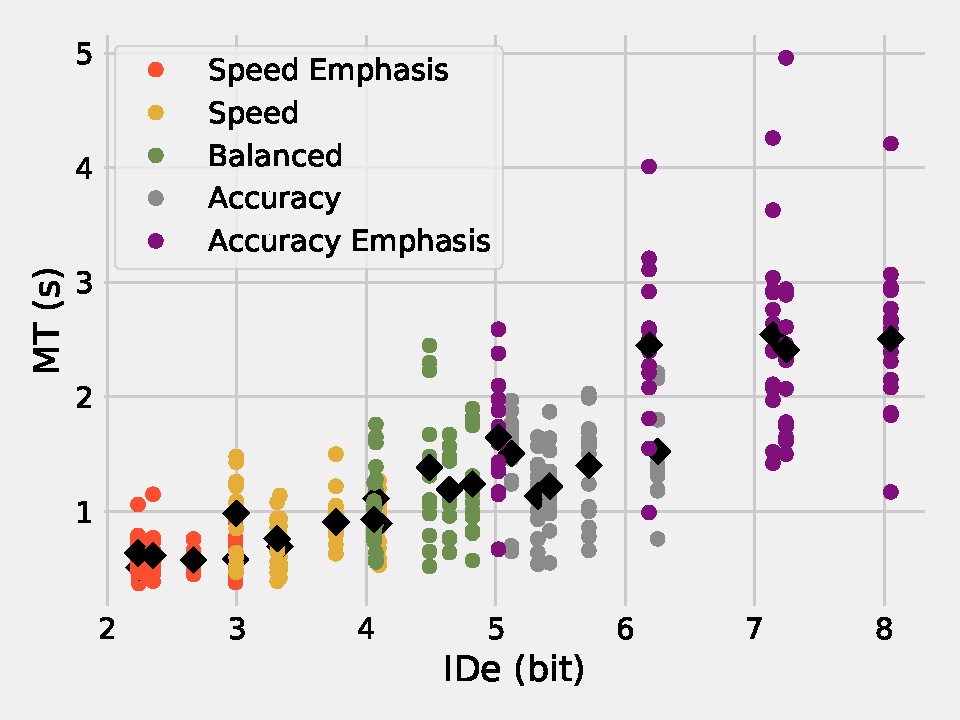
\includegraphics[width=.48\textwidth]{img/fitts_gop_2.pdf} \\
    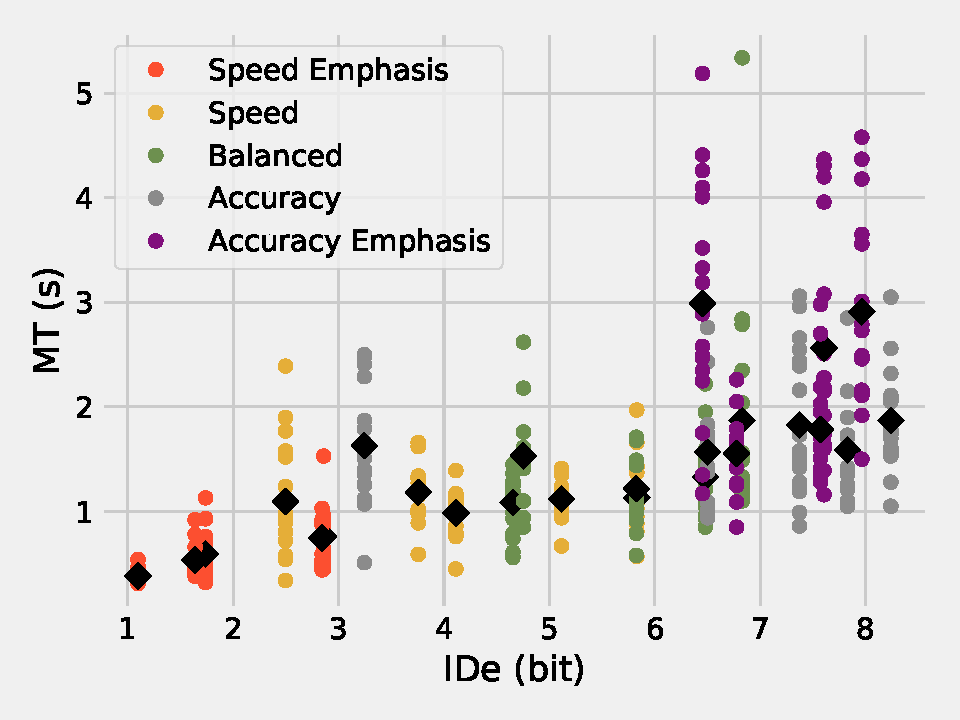
\includegraphics[width=.48\textwidth]{img/fitts_gop_10.pdf}
    \includegraphics[width=.48\textwidth]{img/fitts_gop_16.pdf}
    \caption{The internal consistency of 4 different participants of the GO dataset. Some participants, like the one in the bottom right panel are quite consistent within the same strategy, while some participants, like the one in the bottom left panel have a lot of overlap between strategies.}
\end{figure}


\end{document}